\documentclass[10pt,a4paper]{article}
\usepackage[utf8]{inputenc}
\usepackage[spanish]{babel}
\usepackage{amsmath}
\usepackage{amsfonts}
\usepackage{amssymb}
\usepackage{graphicx}
\usepackage{caption}
\usepackage{subcaption}
\usepackage{listings}
\usepackage{hyperref}
\author{Carlos Manuel Rodríguez Martínez}
\title{Codificador/decodificador de máquinas de Turing}

\begin{document}

\maketitle

\begin{abstract}
   Implementación de codificador/decodificador de máquinas de Turing utilizando el esquema de codificación desarrollado por Penrose.
\end{abstract}

\newpage

\tableofcontents

\newpage

\section{Introducción}
La máquina de Turing es un modelo de máquina capaz de hacer cómputo universal a través de un dispositivo mecánico con un conjunto de reglas de funcionamiento relativamente simple.

Alan Turing nos ofrece la siguiente descripción informal:

\vspace{0.5cm}
``... una ilimitada capacidad de memoria obtenida en la forma de una cinta infinita marcada con cuadrados, en cada uno de los cuales podría imprimirse un símbolo. En cualquier momento hay un símbolo en la máquina; llamado el símbolo leído. La máquina puede alterar el símbolo leído y su comportamiento está en parte determinado por ese símbolo, pero los símbolos en otros lugares de la cinta no afectan el comportamiento de la máquina. Sin embargo, la cinta se puede mover hacia adelante y hacia atrás a través de la máquina, siendo esto una de las operaciones elementales de la máquina. Por lo tanto cualquier símbolo en la cinta puede tener finalmente una oportunidad.''
\vspace{0.5cm}


\section{Definición formal de máquina de Turing}

Formalmente se define a una máquina de Turing como una 7-tupla, $(Q,\Sigma, \Gamma, \delta, q_0, q_{\text{aceptar}},q_{\text{rechazar}})$, donde $Q$, $\Sigma$, $\Gamma$ son conjuntos finitos, y
\begin{enumerate}
	\item $Q$ es el conjunto de estados,
	\item $\Sigma$ es el alfabeto de entrada que no contiene el \textbf{símbolo vacío} \textvisiblespace,
	\item $\Gamma$ es el alfabeto de la cinta, donde $\textvisiblespace \in \Gamma$ y $\Sigma \subseteq \Gamma$,
	\item $\delta : Q \times \Gamma \rightarrow Q \times \Gamma \times \{ L, R \}$ es la función de transición,
	\item $q_0 \in Q$ es el estado inicial,
	\item $q_{\text{aceptar}} \in Q$ es el estado de aceptación, y
	\item $q_{\text{rechazar}} \in Q$ es el estado de rechazo, donde $q_{\text{rechazar}} \neq q_{\text{aceptar}}$.
\end{enumerate}

Esta definición implica la existencia de una configuración de símbolos de la cinta que es específica para cada instante del cómputo que realiza la máquina, junto con el estado asociado a cada configuración y la posición de la cabeza lectora de la máquina. Esta configuración puede representarse por la cadena $u \, q \, v$, donde $u, v \in \Gamma$ son cadenas, y $q \in Q$ es un estado.

Por ejemplo, para una máquina de Turing cuya cinta tiene la cadena $101101111$, se encuentra en el estado $q_7$ y la cabeza se ubica en la posición $4$, esto es sobre el segundo cero, identificando a $u$, y $v$ como $1011$ y $01111$ respectivamente,
\[	
\overbrace{ \underbrace{1011}_\text{u} \underbrace{01111}_\text{v}}^\text{cinta}
\]
la configuración se codifica como $1011q_7 01111$.
Se dice que una máquina de Turing con una configuración $C_1$ produce $C_2$ si se puede transitar de $C_1$ a $C_2$ en un solo paso. Más formalmente, sea $a, b, c \in \Gamma$, $u, v \in \Gamma^*$, y estados $q_i, q_j \in Q$. Sean $u a q_i b v$ y $u q_j a c v$ dos configuraciones,
\[
	u a q_i b v \rightarrow u q_j a c v
\]
sii la función de transición es $\delta(q_i, b) = (q_j, c, L)$. Asimismo,
\[
	u a q_i b v \rightarrow u a c q_j v
\]
sii la función de transición es $\delta(q_i, b) = (q_j, c, R)$.

Existen configuraciones especiales de la máquina donde es relevante hacer una distinción. Sea $M$ una máquina de Turing, que actúa sobre una entrada $w$, se define que:

\begin{itemize}
	\item su \textbf{configuración inicial} es $q_0 w$,
	\item su \textbf{configuración de aceptación} es una cuyo estado sea $q_{\text{aceptar}}$,
	\item su \textbf{configuración de rechazo} es una cuyo estado sea $q_{\text{rechazar}}$,
	\item su \textbf{configuración de interrupción} es o bien una configuración de aceptación o de rechazo.
\end{itemize}

Se dice que $M$ \textbf{acepta} una entrada $w$ si existe una secuencia de configuraciones $C_1, C_2, \dots, C_k$ donde:
\begin{enumerate}
	\item $C_1$ es la configuración inicial de $M$ en  la entrada $w$,
	\item cada $C_i$ produce $C_{i+1}$, y
	\item $C_k$ es una configuración de aceptación.
\end{enumerate}

\subsection{Codificación de Penrose}
En el libro \textit{The Emperor's New Mind: Concerning Computers, Minds and The Laws of Physics} \cite{Penrose} el autor desarrolla un procedimiento para crear una función capaz de mapear del conjunto de los números naturales $\mathbb{N}$ al conjunto de todas las posibles máquinas de Turing con el fin de ofrecer una explicación del \textit{problema del paro}.

\subsubsection{Descripción del programa}
La codificación de Penrose es una manera de asignar un número natural a cada posible máquina de Turing. Para esto se restringe el alfabeto de entrada a un sólo símbolo, de manera que el alfabeto de la cinta es $\Gamma = \{0,1\}$ donde se toma al $0$ como símbolo vacío. Se establece la siguiente notación para la descripción de un programa:
\[
	_{q_i}\textbf{R} \rightarrow _{q_j}\textbf{W}_{D},
\]
donde $q_i$ es el estado de la configuración $i$, $\textbf{R}$ es el símbolo que lee la máquina, $q_j$ es el estado de la configuración $j$, $\textbf{W}$ es el símbolo que escribe la máquina y $D$ es la dirección que puede ser $D = \{L,R\}$. La descripción de un programa se da por medio de la concatenación de instrucciones, por ejemplo:

\begin{align*}
	&_{0}\textbf{0} \rightarrow _{0}\textbf{0}_{R} \\
	&_{0}\textbf{1} \rightarrow _{13}\textbf{1}_{L} \\
	&_{1}\textbf{0} \rightarrow _{65}\textbf{1}_{R} \\
	&_{1}\textbf{1} \rightarrow _{1}\textbf{0}_{R} \\
	&_{2}\textbf{0} \rightarrow _{0}\textbf{1}_{Halt} \\
	&_{2}\textbf{1} \rightarrow _{66}\textbf{1}_{L} \\
	& \vdots \\
	&_{258}\textbf{1} \rightarrow _{0}\textbf{0}_{Halt} \\
	&_{259}\textbf{0} \rightarrow _{97}\textbf{1}_{R} \\
	&_{259}\textbf{1} \rightarrow _{0}\textbf{0}_{Halt}
\end{align*}

Esta notación para la descripción de un programa resulta conveniente para la lectura humana en la interpretación de un algoritmo, sin embargo si lo que se busca es la notación más compacta es posible hacer varias mejoras.

\subsubsection{Procedimiento de codificación}
Para el procedimiento de codificación de la máquina de Turing según la notación de Penrose se busca eliminar todo tipo de redundancia a fin de encontrar la manera más compacta de expresar el funcionamiento. Primero, la información de la columna izquierda es redundante, la posición de cada instrucción es suficiente para determinar a qué estado y símbolo corresponde. Podemos expresar el programa de la siguiente manera;
\[
	_{0}\textbf{0}_{R}, _{13}\textbf{1}_{L}, _{65}\textbf{1}_{R}, _{1}\textbf{0}_{R}, \dots, _{97}\textbf{1}_{R}, _{0}\textbf{0}_{Halt}.
\]
Se puede notar también que las comas y la notación $_{x}y_z$ son innecesarias, incluso sin ellas es posible distinguir los estados de los símbolos de entrada sin señalamiento adicional debido a que los símbolos de entrada siempre son seguidos por  L,R, o H.
\[
	0 \textbf{0} R 13 \textbf{1} L 65 \textbf{1} R 1 \textbf{0} R \dots 97 \textbf{1} R 0 \textbf{0} H
\]

Si deseamos restringir la cantidad de símbolos utilizados en la descripción de un programa podemos hacer el uso de la codificación binaria para los estados
\[
	_{0}\textbf{0}_{R}, _{1101}\textbf{1}_{L}, _{1000001}\textbf{1}_{R}, _{1}\textbf{0}_{R}, \dots, _{1100001}\textbf{1}_{R}, _{0}\textbf{0}_{Halt}
\]
o en forma más compacta
\[
	0 \textbf{0} R \quad 1101 \textbf{1} L \quad 1000001 \textbf{1} R \quad 1 \textbf{0} R \quad \dots \quad 1100001 \textbf{1} R \quad 0 \textbf{0} H
\]

Es posible simplificar esta representación quitando todos los dígitos innecesarios. Por ejemplo, $0 \textbf{0}$ se puede omitir por completo sin perder información y $0 \textbf{1}$ es posible dejarlo sólo como $1$. También, por definición de la notación utilizada, toda máquina de Turing comienza con una instrucción que mueve la cabeza lectora hacia la derecha. Es posible omitir este símbolo. Aquí se está asumiendo que todas las máquinas de Turing comienzan con la instrucción $0 \textbf{0} R$, esto asegura que el dispositivo puede empezar a funcionar arbitrariamente lejos hacia la izquierda y llegará siempre a la primera sobre la cinta.
\[
	1101 \textbf{1} L \quad 1000001 \textbf{1} R \quad 1 \textbf{0} R \quad \dots \quad 1100001 \textbf{1} R \quad H
\]
A este procedimiento que codifica el programa en la menor cantidad de símbolos se le llamará \textit{simplificación}.

A partir de la simplificación anterior, es posible codificar esta secuencia en sólo dos símbolos $\{0,1\}$ por medio de la siguiente regla de sustitución
\begin{align*}
	&0 \rightarrow 0,\\
	&1 \rightarrow 10,\\
	&R \rightarrow 110,\\
	&L \rightarrow 1110,\\
	&H \rightarrow 11110.
\end{align*}

El motivo de esta forma de codificación tiene origen en la entropía de la información. Bajo la suposición de que la cinta comienza con un número infinito de ceros que representan espacios vacíos y se mueve inicialmente hacia la derecha, es de esperar que los espacios vacíos $0$ sean más frecuentes en la cinta que las marcas $1$, asimismo el símbolo $R$ será más frecuente que $L$. Es por esto que en la codificación anterior se utiliza menor cantidad de dígitos para describir a los símbolos más frecuentes y viceversa. Esto nos asegura que la codificación minimice la entropía de la información.

Aplicando esta codificación a los símbolos no numéricos de la secuencia anterior queda lo siguiente, donde los dígitos se han encerrado entre paréntesis:
\[
	(1101) \; (1) \; 1110 \; (1000001) \; (1) \; 110 \; (1) \; (0) \; 110 \; \dots \; (1100001) \; (1) \; 110 \; 11110
\]
Aplicando la codificación a los dígitos queda terminada la segunda parte del proceso que se denomina \textit{expansión}.
\[
	101001010111010000001010110100110 \dots 10100000101011011110
\]
Por último, se puede borrar el $110$ final de la secuencia ya que siempre termina con los símbolos $L$, $R$ o $H$, que también terminan en $110$. A este tercer paso se le llama \textit{corte}.
\[
	101001010111010000001010110100110 \dots 10100000101011011
\]
El número $n$ resultante de este proceso es el número natural asociado con la máquina de Turing $T_n$. Por conveniencia se utilizará la representación decimal de $n$.

\subsubsection{Procedimiento de decodificación}
El procedimiento de decodificación consiste en deshacer los pasos del procedimiento de codificación. El procedimiento se puede dividir en tres etapas.

\begin{enumerate}
	\item \textbf{Preprocesamiento:} Se convierte el número $n$ de entrada a su representación binaria añadiendo al final la secuencia $110$ que fue eliminada durante del proceso de codificación.
	\item \textbf{Análisis léxico:} Una vez recuperada la secuencia binaria es necesario identificar los \textit{tokens} que la componen. La tabla de equivalencia entre dígitos y \textit{tokens} es inversa al proceso de codificación:
\begin{align*}
	&0 \rightarrow 0,\\
	&10 \rightarrow 1,\\
	&110 \rightarrow R,\\
	&1110 \rightarrow L,\\
	&11110 \rightarrow H.
\end{align*}
Una vez terminado el procedimiento se agregan los \textit{tokens} $00R$ al inicio del programa, ya que esta es la instrucción inicial común a todas las máquinas.
	\item \textbf{Parser:} Por último se agrupan los \textit{tokens} para formar las instrucciones que definen al programa. Es necesario reconstruir las instrucciones incluyendo los estados $0$ y $1$ que fueron eliminados. Añadiendo la parte izquierda de las instrucciones queda terminada la reconstrucción del programa.
\end{enumerate}

\subsubsection{Descripción de codificación en cinta de los datos numéricos}
Para lograr la universalidad de cómputo de la máquina de Turing es necesario encontrar una manera de codificar los valores numéricos que se le pasan como argumento a cada algoritmo. Para codificar se convierte el número a binario y se hará un procedimiento de expansión, es decir se hará el reemplazo:
\begin{align*}
	&0 \rightarrow 0,\\
	&1 \rightarrow 10.
\end{align*}
Para separar cada argumento siempre se añadirá un símbolo que represente el token coma, esto es $, \rightarrow 110$. Como ejemplo de esta representación el número $167$ quedará representado en la cinta como:

\[
	1001000101010110.
\]

\subsection{Representaciones alternativas}
Una forma alternativa de representar cada configuración de la máquina consiste en representar cada estado con una flecha y cada elemento de celda por un color. Esto nos daría que la representación equivalente de la configuración $1011q_7 01111$ es:
\begin{figure}[h!tb!]
	\centering
	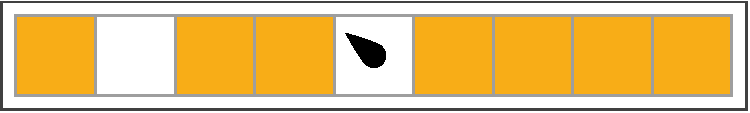
\includegraphics[scale=0.38]{../img/example_initial.pdf}
\end{figure}

Esta representación fue la utilizada por Wolfram en su libro ANKS \cite{Wolfram2002}. La ventaja de utilizar esta representación es que nos permite obtener una intuición rápida de las reglas que definen a la máquina de Turing. Por ejemplo, podemos definir a la máquina de Turing \textbf{UN+1} de $2$ estados y con número $177642$ cuya descripción en la notación de Penrose es:

\begin{align*}
	&_{0}\textbf{0} \rightarrow _{0}\textbf{0}_L \\
	&_{1}\textbf{0} \rightarrow _{1}\textbf{1}_R \\
	&_{0}\textbf{1} \rightarrow _{1}\textbf{0}_H \\
	&_{1}\textbf{1} \rightarrow _{1}\textbf{1}_R
\end{align*}

de la siguiente manera:
\begin{figure}[h!tb!]
	\centering
	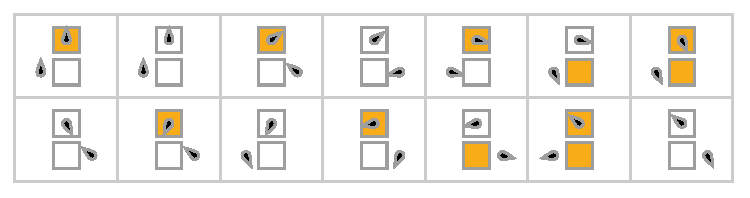
\includegraphics[scale=0.68]{../img/example_rules.pdf}
	\caption{Reglas de evolución de la maquina \textbf{UN+1}.}
	\label{fig:un1rules}
\end{figure}

Con esta notación es fácil visualizar la ejecución de la máquina utilizando la misma representación de flechas:

\begin{figure}[h!tb!]
	\centering
	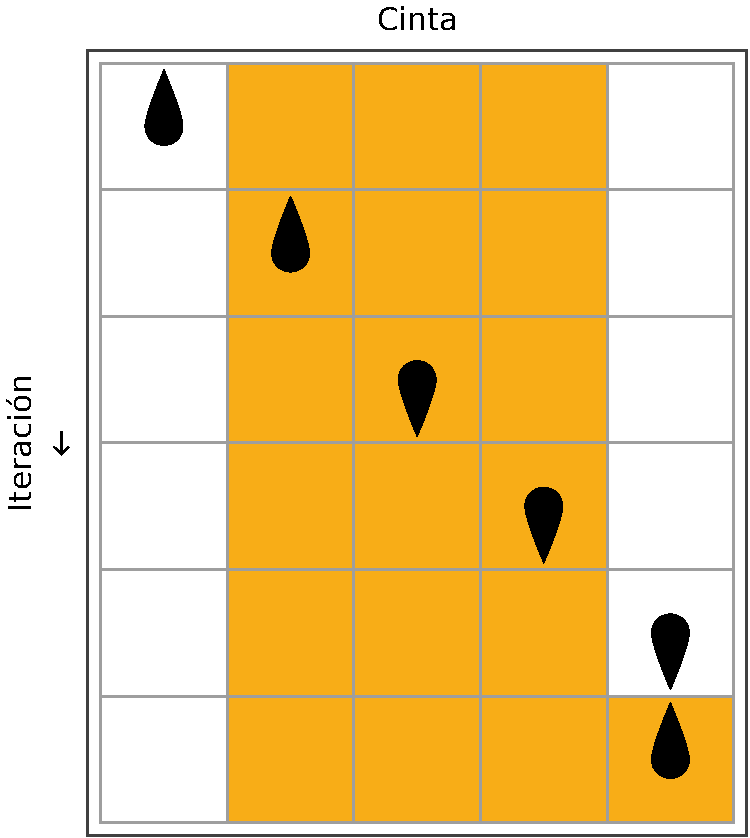
\includegraphics[scale=0.40]{../img/example_evolution.pdf}
	\caption{Evolución temporal de la maquina \textbf{UN+1}.}
	\label{fig:un1evolution}
\end{figure}

Otra representación útil de la máquina de Turing consiste en utilizar un grafo cuyos nodos son los estados y los vértices representan las transiciones. Así, la máquina \textbf{UN+1} quedaría representada como se muestra en la figura \ref{fig:un1graph}.
\begin{figure}[h!tb!]
	\centering
	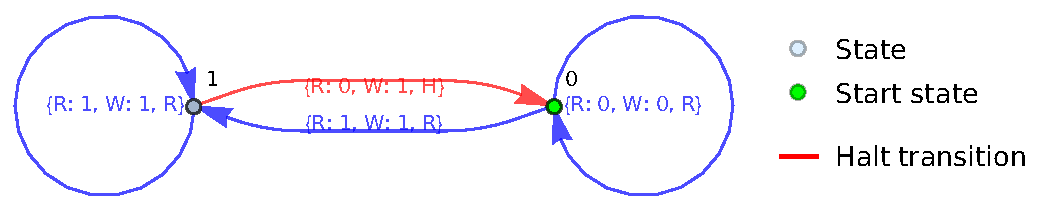
\includegraphics[scale=0.48]{../img/un1_graph.pdf}
	\caption{Representación de grafo de la maquina \textbf{UN+1}.}
	\label{fig:un1graph}
\end{figure}

\section{Implementación}
La implementación del proyecto se realizó utilizando el lenguaje Wolfram. La justificación para el uso de este lenguaje es debido a las facilidades preexistentes en las bibliotecas estándar. Históricamente el software Mathematica fue desarrollado como una herramienta de investigación de sistemas capaces de exhibir complejidad como autómatas celulares, sistemas de sustitución y máquinas abstractas, entre las cuales se encuentra la máquina de Turing.

\subsection{Rutinas de codificación}
Para realizar la codificación primero se estableció una notación para representar el programa por medio de una lista de asociaciones (similar a los diccionarios en Python).

\begin{figure}[h!tb!]
	\centering
	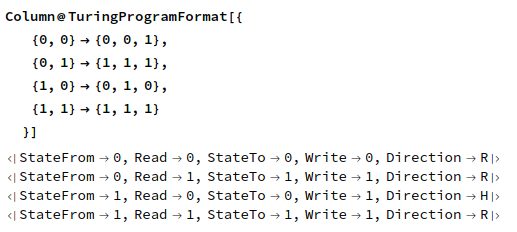
\includegraphics[scale=0.45]{../img/association.png}
\end{figure}

Las funciones de codificación hacen uso de esta representación estructurada para aplicar las reglas de codificación descritas en la sección anterior. Se definen varias reglas que actúan sobre formas diferentes de cada instrucción.

\begin{figure}[h!tb!]
	\centering
	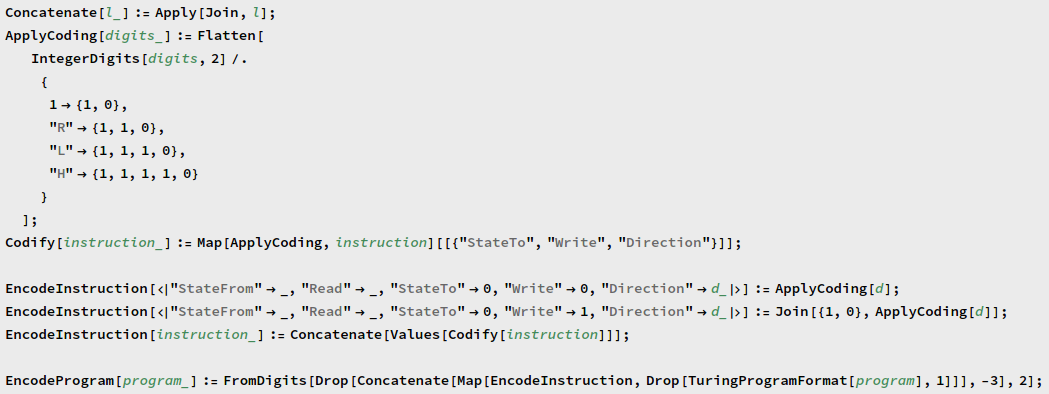
\includegraphics[scale=0.35]{../img/encoding.png}
\end{figure}

Aplicando las reglas, cortando información redundante y transformando la secuencia resultante a un número en base decimal se obtiene el resultado.

\subsection{Rutinas de decodificación}
La decodificación tiene una implementación más complicada debido a que es necesario reconstruir un programa que ha sido simplificado durante el procedimiento de codificación. Se implementó creando un parser capaz de reconocer los \textit{tokens} e instrucciones de cada programa,

\begin{figure}[h!tb!]
	\centering
	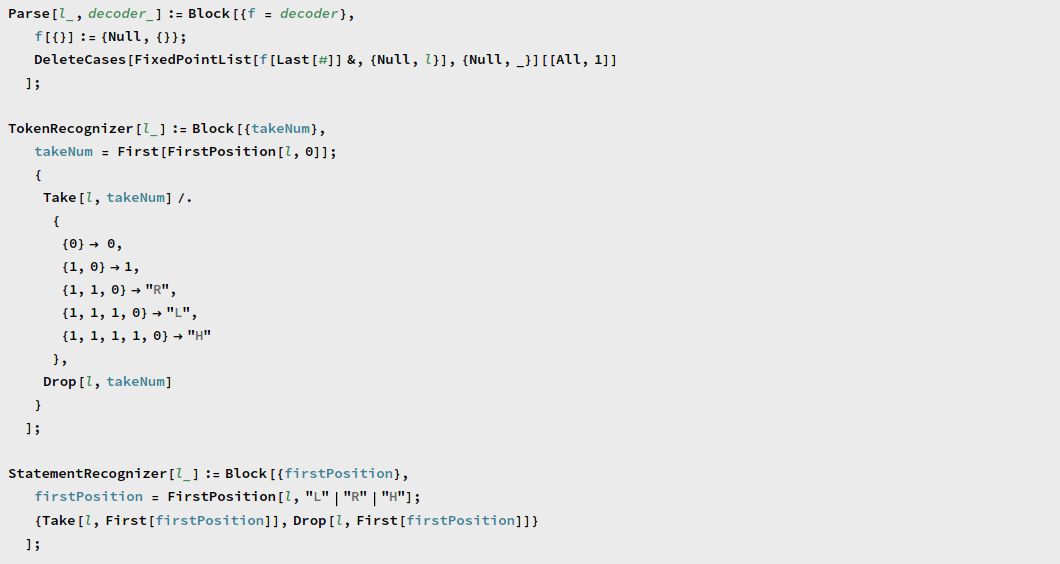
\includegraphics[scale=0.35]{../img/decoding_parser.png}
\end{figure}

y por último se procesa el resultado para obtener la reconstrucción del programa:
\begin{figure}[h!tb!]
	\centering
	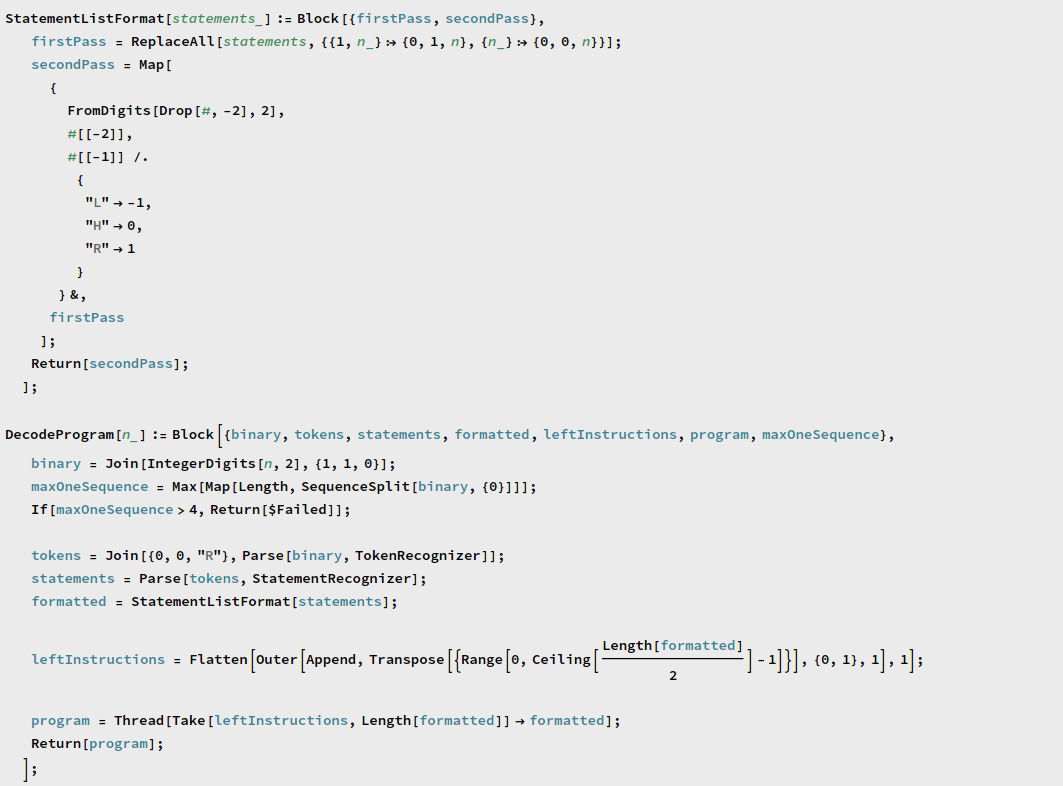
\includegraphics[scale=0.35]{../img/decoding_frontend.png}
\end{figure}

\clearpage

\section{Máquinas interesantes}
Al tener una función que mapea los números naturales $\mathbb{N}$ es posible estudiar y ejecutar las máquinas generadas por cualquier número arbitrario. Esto no implica que todas las máquinas sean interesantes o realicen algo útil.

\subsection{Primeras 12 máquinas}
Al generar las primeras 12 máquinas que se muestran en la figura \ref{fig:first12} y estudiar su comportamiento es notable que casi ninguna realiza algo útil, lo más que logran es cambiar una celda o realizar una acción simple eternamente. Algunas máquinas como la 7 ni siquiera están especificadas correctamente.

\begin{figure}[h!tb!]
	\centering
	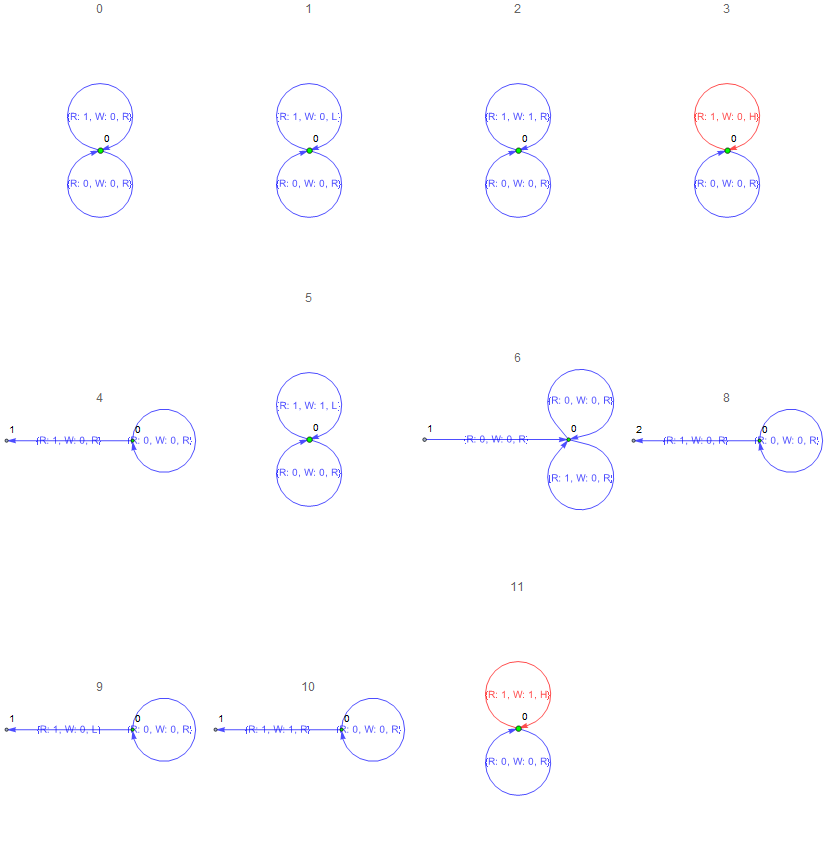
\includegraphics[scale=0.48]{../img/first10}
	\caption{Representación de grafo de las primeras 12 máquinas de Turing.}
	\label{fig:first12}
\end{figure}

\clearpage

\subsection{UN+1}
La máquina \textbf{UN+1} codificada como
\begin{lstlisting}
un1 = 177642
\end{lstlisting}
es una de las máquinas funcionales más simples. Su comportamiento consiste en avanzar la cabeza lectora hacia adelante hasta encontrar el último cero, el cual reemplaza por $1$ y termina la ejecución. Esto tiene como efecto que si la cinta contiene un número codificado en unario, el añadir un $1$ al final suma una unidad.

\begin{figure}[htb!]
          \begin{subfigure}[b]{0.48\textwidth}
            \centering 
            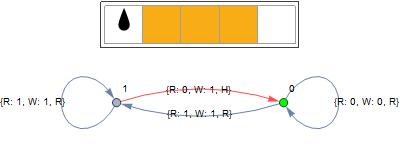
\includegraphics[width=\textwidth]{../img/un1/1}
            \caption{Iteración 1}
          \end{subfigure}
                  \hfill
          \begin{subfigure}[b]{0.475\textwidth}
            \centering 
            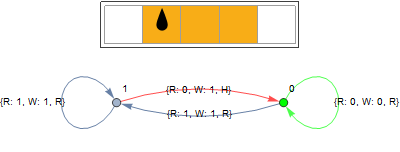
\includegraphics[width=\textwidth]{../img/un1/2}
            \caption{Iteración 2}
          \end{subfigure}
        \vskip\baselineskip
        \centering
        \begin{subfigure}[b]{0.475\textwidth}
            \centering
            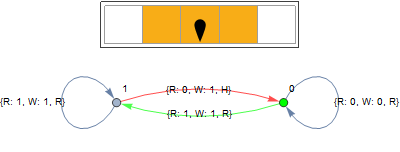
\includegraphics[width=\textwidth]{../img/un1/3}
            \caption{Iteración 3}
        \end{subfigure}
        \hfill
        \begin{subfigure}[b]{0.475\textwidth}
            \centering 
            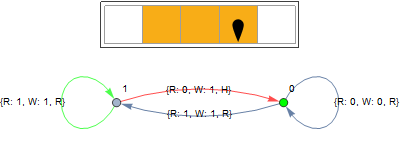
\includegraphics[width=\textwidth]{../img/un1/4}
            \caption{Iteración 4}
        \end{subfigure}
        
        \vskip\baselineskip
        \centering
        \begin{subfigure}[b]{0.475\textwidth}
            \centering
            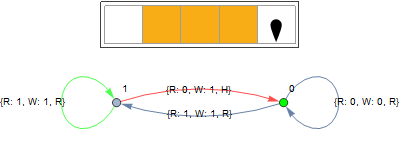
\includegraphics[width=\textwidth]{../img/un1/5}
            \caption{Iteración 5}
        \end{subfigure}
        \caption{Ejecución de \textbf{UN+1} sobre el argumento $3$ codificado en unario.}
\end{figure}

\subsection{XN+1}
La máquina \textbf{XN+1} codificada como
\begin{lstlisting}
xn1 = 450813704461563958982113775643437908
\end{lstlisting}
realiza un procedimiento análogo a \textbf{UN+1} pero actuando sobre un número codificado en la notación binaria expandida. La complejidad adicional de la máquina se refleja en las operaciones que debe realizar para manejar la codificación, lo cual genera una máquina más complicada que \textbf{UN+1}.

\begin{figure}[htb!]
          \begin{subfigure}[b]{0.48\textwidth}
            \centering 
            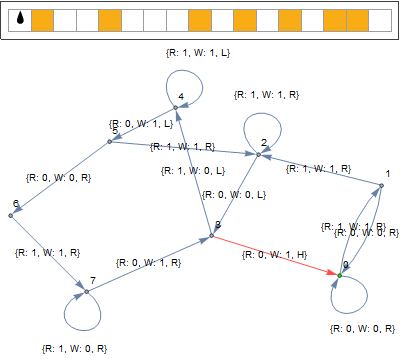
\includegraphics[width=0.8\textwidth]{../img/xn1/1}
            \caption{Iteración 1}
          \end{subfigure}
          \hfill
          \begin{subfigure}[b]{0.475\textwidth}
            \centering 
            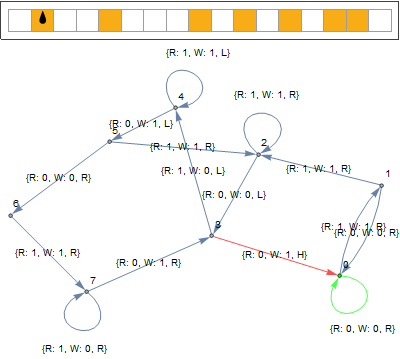
\includegraphics[width=0.8\textwidth]{../img/xn1/2}
            \caption{Iteración 2}
          \end{subfigure}
        \vskip\baselineskip
        \centering
        \begin{subfigure}[b]{0.475\textwidth}
            \centering
            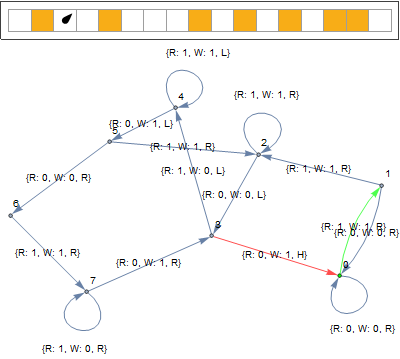
\includegraphics[width=0.8\textwidth]{../img/xn1/3}
            \caption{Iteración 3}
        \end{subfigure}
        \hfill
        \begin{subfigure}[b]{0.475\textwidth}
            \centering 
            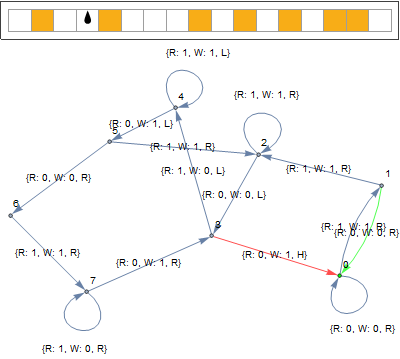
\includegraphics[width=0.8\textwidth]{../img/xn1/4}
            \caption{Iteración 4}
        \end{subfigure}
        
        \vskip\baselineskip
        \centering
        \begin{subfigure}[b]{0.475\textwidth}
            \centering
            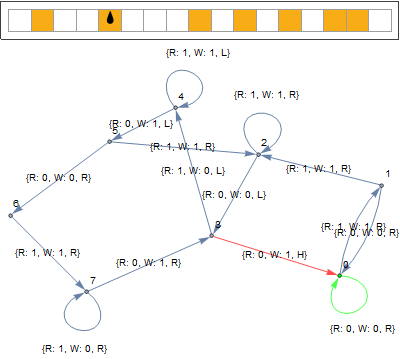
\includegraphics[width=0.8\textwidth]{../img/xn1/5}
            \caption{Iteración 5}
        \end{subfigure}
        \hfill
        \begin{subfigure}[b]{0.475\textwidth}
            \centering 
            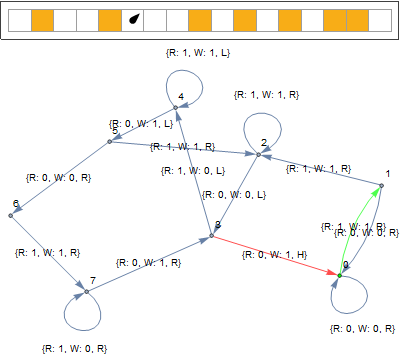
\includegraphics[width=0.8\textwidth]{../img/xn1/6}
            \caption{Iteración 6}
        \end{subfigure}
        
        \vskip\baselineskip
        \centering
        \begin{subfigure}[b]{0.475\textwidth}
            \centering
            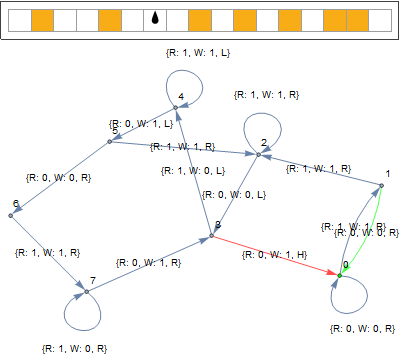
\includegraphics[width=0.8\textwidth]{../img/xn1/7}
            \caption{Iteración 7}
        \end{subfigure}
        \hfill
        \begin{subfigure}[b]{0.475\textwidth}
            \centering 
            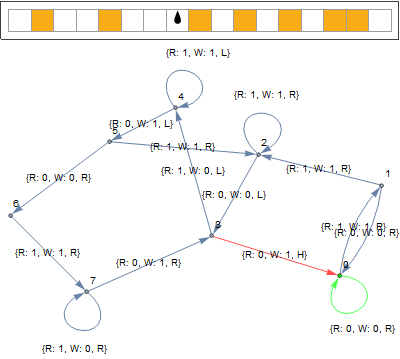
\includegraphics[width=0.8\textwidth]{../img/xn1/8}
            \caption{Iteración 8}
        \end{subfigure}
        \caption{Primeras 8 iteraciones de la ejecución de \textbf{XN+1} sobre el argumento $167$ codificado en binario expandido.}
\end{figure}

\clearpage

\subsection{UTM}
La máquina universal de Turing \textbf{UTM} que actúa sobre una cinta con los argumentos $n$ y $m$ e imita el comportamiento de la máquina $T_n$ actuando sobre $m$,
\[
	U(n,m) = T_n(m)
\]

es la máquina número

\begin{lstlisting}
u = 724485533533931757719839503961571123795236067255655963
1108144796606505059404241090310483613632359365644443458382
2268832787676265561446928141177150178425517075540856576897
5334635694247848859704693472573998858228382779529468346052
1061169835945938791885546326440925525505820555989451890716
5374148960330967530204315536250349845298323206515830476641
4213070881932971723415105698026273468642992183817215733348
2823073453713421475059740345184372359593090640024321077342
1788514927607975976344151230795863963544922691594796546147
1134570014504816733756217257346452273105448298078496512698
8788964569760906634204477989021914437932830019493570963921
7039048332708825962013017737272027186259199144282754374223
5135567513408422229988937441053430547104436869587640517812
8019437530813870639942772823156425289237514565443899052780
7932411448261423572861931183326106561227555318102075110853
3763380603108236167504563585216421486954234718742643754442
8790062485827091240422076538754264454133451748566291574299
9095026230097337381377241621727477236102067868540028935660
8569682262014198248621698902609130940298570600174300670086
8967590344734174127874255812015493663938996905817738591654
0553567040928213322216314109787108145997866959970450968184
1906299443656015145490488092208448003482249207730403043188
4298993931352668823496621019471619107014619685231928474820
3449589770955356110702758174873332729667899879847328409819
0764851272631001740166787363477605857245036964434897992034
4899974556624029374876688397514044516657077500605138839916
6881407254554466522205072426239237921152531816251253630509
3172863142200406457130527580230766518335199568913974813750
4926429605010013651980186945639498.
\end{lstlisting}

Para representar los números $n$ y $m$ en la cinta se codifican colocando el número $m$ en binario, se añade la secuencia $111110$ que actúa como una coma, se coloca el número $m$ en binario y por último se agrega la secuencia $10\dots$ donde se asume que el resto de la cinta contiene un número infinito de ceros.

Al ejecutar la máquina universal la cabeza lectora va realizando el cómputo cambiando tanto las celdas que contienen el programa $n$ como las celdas anteriores. Una vez que la máquina se detiene, el resultado del cómputo son todas las celdas a la izquierda de la última posición de la cabeza lectora.

El grafo de la máquina se muestra en la figura \ref{fig:utmGraph}. Es notable la complejidad de la máquina universal que se debe en parte a las diferentes subrutinas que debe realizar a fin de imitar el comportamiento de la máquina que se le pasa como argumento.

\begin{figure}[h!tb!]
	\centering
	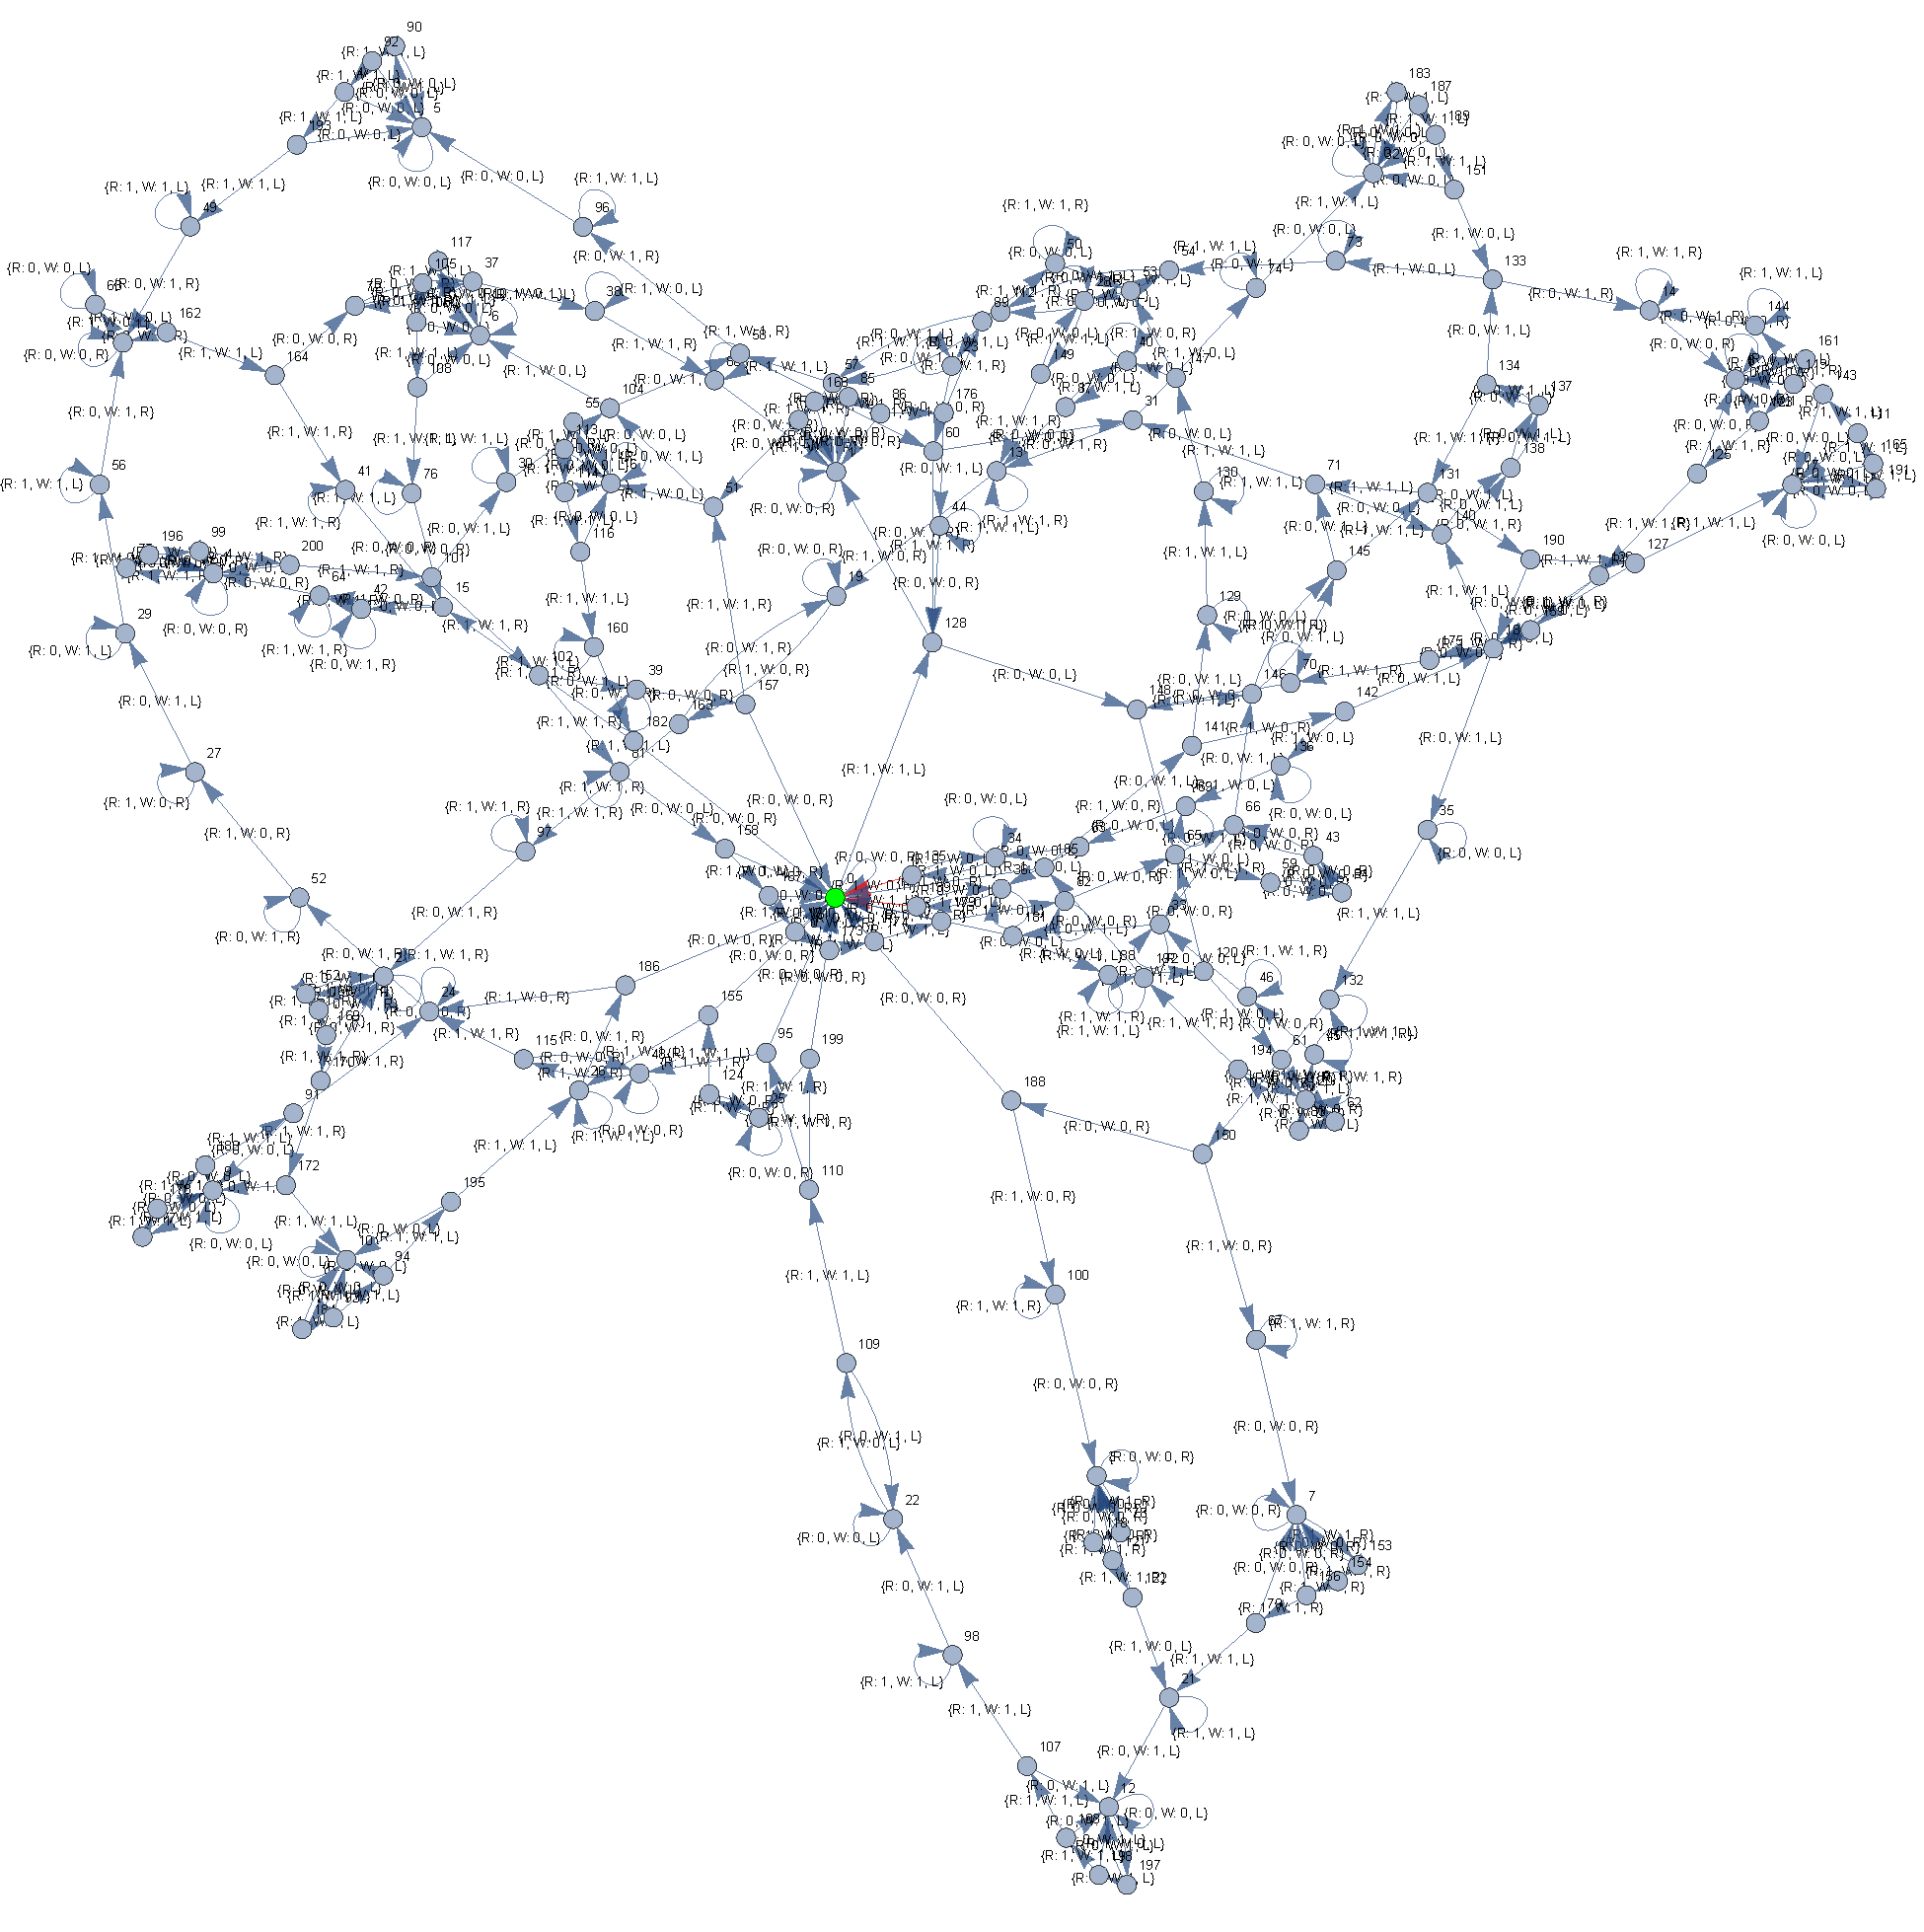
\includegraphics[scale=0.42]{../img/utm_graph.pdf}
	\caption{Grafo de UTM.}
	\label{fig:utmGraph}
\end{figure}

La visualización de una UTM ejecutando el algoritmo \textbf{UN+1} se encuentra disponible en formato de vídeo y se puede visualizar en la siguiente ubicación:

\url{https://youtu.be/L61pt9tTSKs}

\clearpage

\subsection{Descripción de su funcionamiento}
Penrose no ofrece ninguna descripción del funcionamiento de la máquina universal, pero es posible identificar el funcionamiento principal haciendo uso de la representación de grafo de la máquina. Se identificaron dos secciones diferenciadas durante la ejecución de \textbf{UN+1} sobre el argumento $m = 3$. Primero la cabeza lectora se mueve hacia la derecha interpretando las instrucciones y llegando hasta la primera posición del número $m$ (\textit{fetch}), para posteriormente iniciar un camino de regreso que finaliza al dejar (o no) una marca a la izquierda de $n$ (\textit{write}), que es el resultado de la emulación de la máquina \textbf{UN+1} sobre la primera celda. El proceso se repite de manera análoga durante la ejecución de los 5 pasos que realiza la máquina.

En la figura \ref{fig:fetch} se muestran los estados y transiciones involucradas en el proceso \textit{fetch}, y asimismo se muestra en \ref{fig:write} los estados y transiciones involucrados en el proceso \textit{write}.

\begin{figure}[h!tb!]
	\centering
	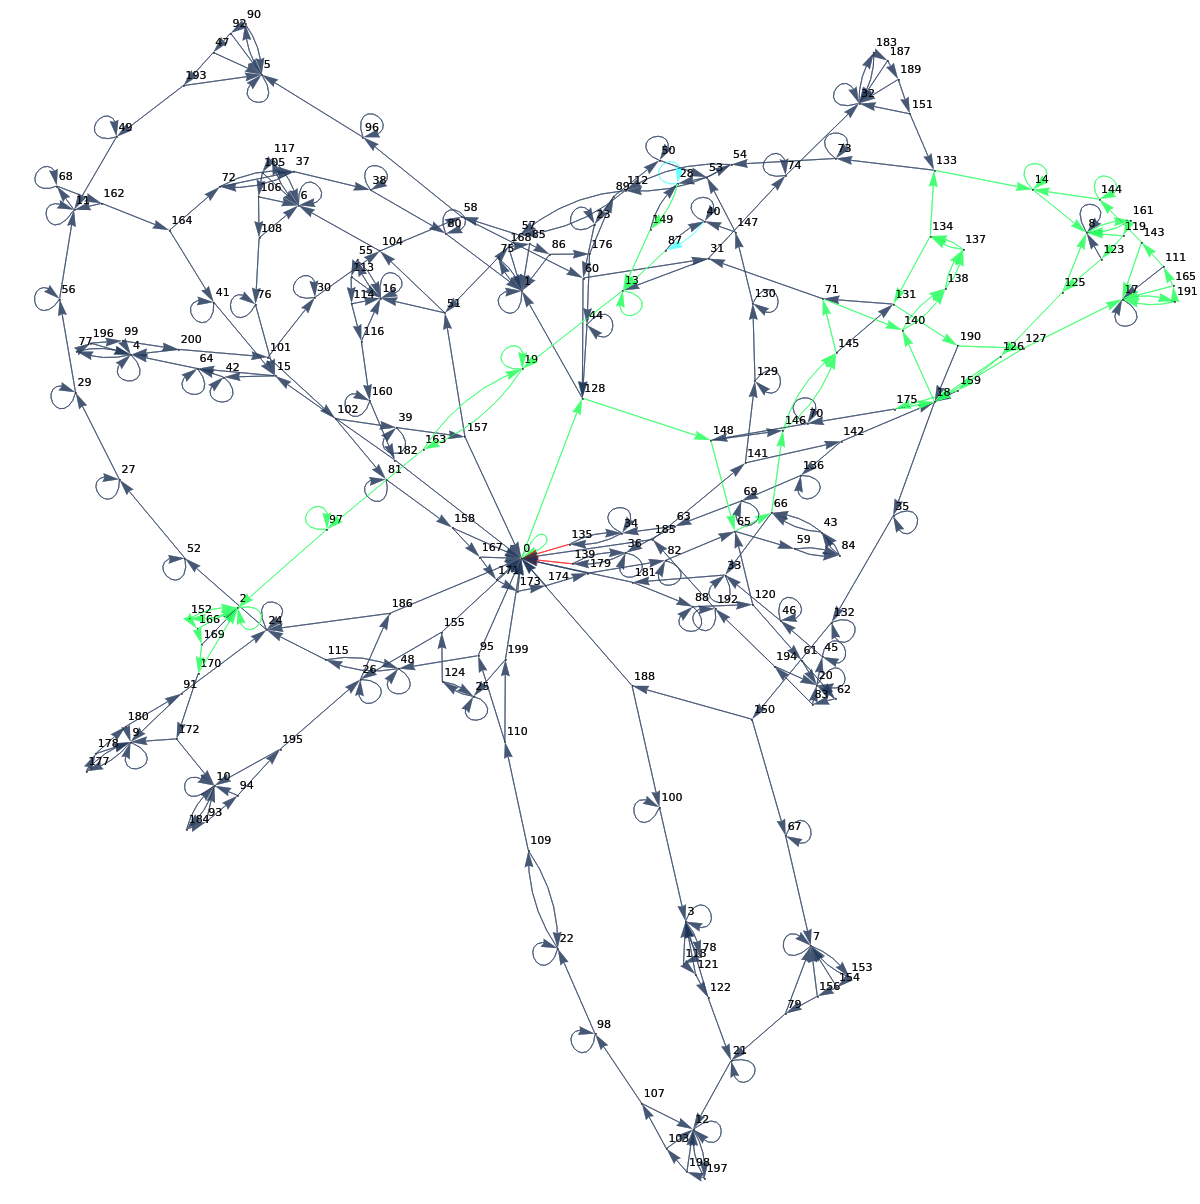
\includegraphics[scale=0.35]{../img/fetchSection.png}
	\caption{Sección \textit{fetch}}
	\label{fig:fetch}
\end{figure}

\begin{figure}[h!tb!]
	\centering
	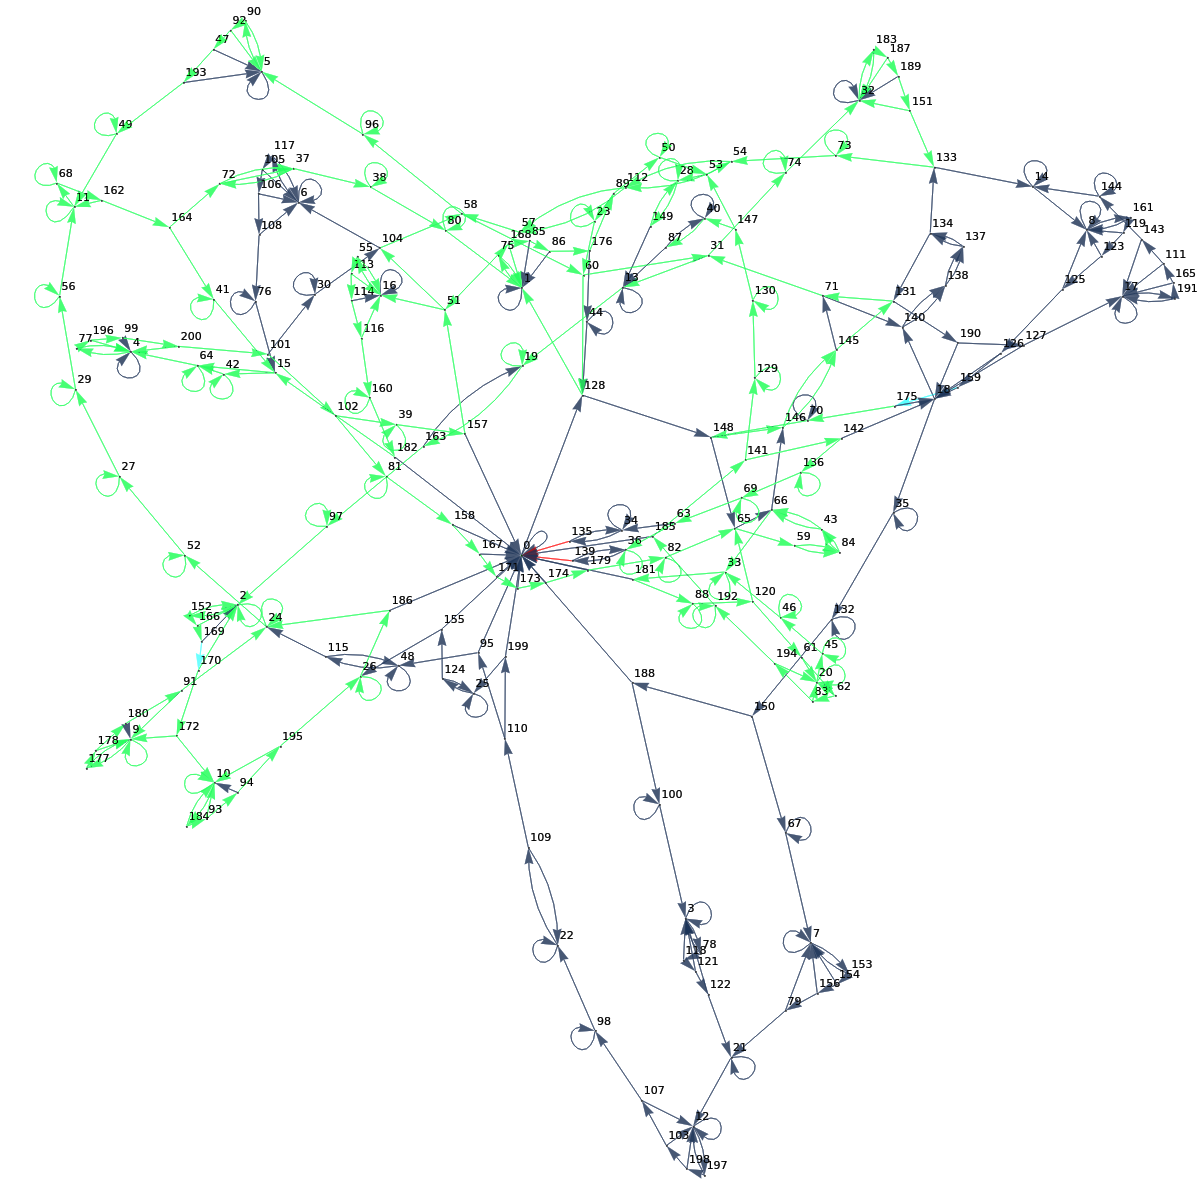
\includegraphics[scale=0.35]{../img/writeSection.png}
	\caption{Sección \textit{write}}
	\label{fig:write}
\end{figure}

\clearpage

\section{Conclusión}
Tener una función capaz de hacer un mapeo de los números naturales $\mathbb{N}$ a las máquinas de Turing y viceversa provee de un método interesante para representar la complejidad de los algoritmos. De una manera muy burda pudo observarse que para codificar comportamientos más sofisticados o útiles (donde la utilidad se define de una manera antropocéntrica) es necesario utilizar números extremadamente grandes. Esto reduce las posibilidades de encontrar una máquina interesante tomando un número natural al azar ya que la mayoría de ellas no realiza ninguna acción útil. Al mismo tiempo la codificación nos permite obtener un indicador numérico de la sofistificación de un algoritmo en particular, y esto puede ser explorado a futuro implementando rutinas capaces de codificar en un número natural programas compilados para ser ejecutados en máquinas de Turing utilizando el lenguaje de programación y compilador del proyecto \textit{Laconic} \cite{Yedidia2016}.

\nocite*

%\newpage
\bibliography{Referencias}{}
\bibliographystyle{plain}

\end{document}